\documentclass[a4paper, 12pt]{article}

%•	Lucrarea se recomandă a avea între 30 și 60 de pagini
%•	Format: A4, fonturi de 12pt, distanță de 1.5 între rânduri
%•	Obligatoriu paginile sunt numerotate
%•	Capitolele vor începe pe pagină nouă
% margini: top=2.5cm,left=3cm,right=2.5cm,bottom=2.5cm
\usepackage{comment}
\usepackage{setspace}

% for bibliography
\usepackage[english]{babel}
\usepackage[nottoc]{tocbibind}
% subfigure
\usepackage{subcaption}

% for clicking on a cite leading to bibliography
\usepackage{hyperref}
\hypersetup{
    colorlinks=true,
    linkcolor=black,
    citecolor=blue,
    urlcolor=blue,
    filecolor=blue, 
}
% specificatii in legatura cu margini
\usepackage[top=2.5cm,left=3cm,right=2.5cm,bottom=2.5cm]{geometry}

\usepackage{graphicx}

% Redefine \maketitle to customize title layout
\makeatletter
\renewcommand{\maketitle}{
    \begin{center}
            \normalsize{BABEŞ-BOLYAI UNIVERSITY CLUJ-NAPOCA}\par % University name
            \normalsize{FACULTY OF MATHEMATICS AND COMPUTER SCIENCE}\par % Faculty name
            \normalsize{COMPUTER SCIENCE IN ROMANIAN SPECIALIZATION}\par
        \vspace{21em} % Vertical space

        {\LARGE\@title\par} % Title in large font
        \vspace{21em} % Vertical space

        \textbf{Supervisor}\hspace{20em}\textbf{Author}\par
        Prof.dr. Horia F. Pop\hspace{16em}{\large\@author\par} % Author
        \vspace{3em} % Vertical space

        {\large\@date\par} % Date
    \end{center}
}
\makeatother

\title{
    DIPLOMA THESIS \\
    Alzheimer's Disease Detection
}
\author{Ichim Ștefan}
\date{2024}

% Set line spacing to 1.5
\onehalfspacing

\begin{document}

% title page
\maketitle
\newpage

% ------------------------------------ABSTRACT--------------------------------------
% abstract page
\begin{abstract}
    Lorem ipsum Lorem ipsum Lorem ipsum Lorem ipsum
    Lorem ipsum Lorem ipsum Lorem ipsum Lorem ipsum
    Lorem ipsum Lorem ipsum Lorem ipsum Lorem ipsum
    Lorem ipsum Lorem ipsum Lorem ipsum Lorem ipsum
    Lorem ipsum Lorem ipsum Lorem ipsum Lorem ipsum
    Lorem ipsum Lorem ipsum Lorem ipsum Lorem ipsum
    Lorem ipsum Lorem ipsum Lorem ipsum Lorem ipsum
    Lorem ipsum Lorem ipsum Lorem ipsum Lorem ipsum
\end{abstract}
\newpage

% ------------------------------------CONTENTS--------------------------------------
\tableofcontents
\newpage

% ----------------------------------INTRODUCTION------------------------------------
\section{Introduction}
There is no denying that humanity stands at a previously inconceivable point in healthcare and medicine,
which naturally have led to hindrances in senescence, populations increasingly reaching older stages of life.
Furthermore, studies which take into account multiple case scenarios show that population is expected to reach
9.2 billion by the age of 2050, leading to an uprise of 21\% in the elderly. \cite{KC2017181}

With that being said, researchers' concern has has taken a turn towards diseases occurring at these later
parts of human lives, some of them considered treatable while others less so.
One of such disorders is Alzheimer's Disease, or AD, considered to be the most likely predecessor of dementia.
Alzheimer's Disease is a brain disease, neurodegenerative, which in time diminishes cognitive skills such as memory,
thinking and speaking, and in due course even removes the ability of accomplishing simple activities vital to one's
daily life.
On top of that, it is an incurable disorder, which only underlines even further the reasons why early
detection stand of such great importance, so that appropriate actions can be taken by both the medical team
and the one diagnosed, along with their relatives and close ones.

\subsection{Disease Summary}

The brain of a healthy human represents a cluster of neurons by the number of bilions which together amount to
what actions and reactions we have, through a process of signal propagating.
Through our sensory mechanism, which includes hearing and seeing, receptors carry out the tasks of sending signals
(Fig \ref{fig:neuron-communication}) using designated channels all the way to the neurons inside the brain, where new
specific signals are formed and sent back, resulting in what we call actions. \cite{Sivadas2020HowDM}

\begin{figure}[htbp]
    \centering
    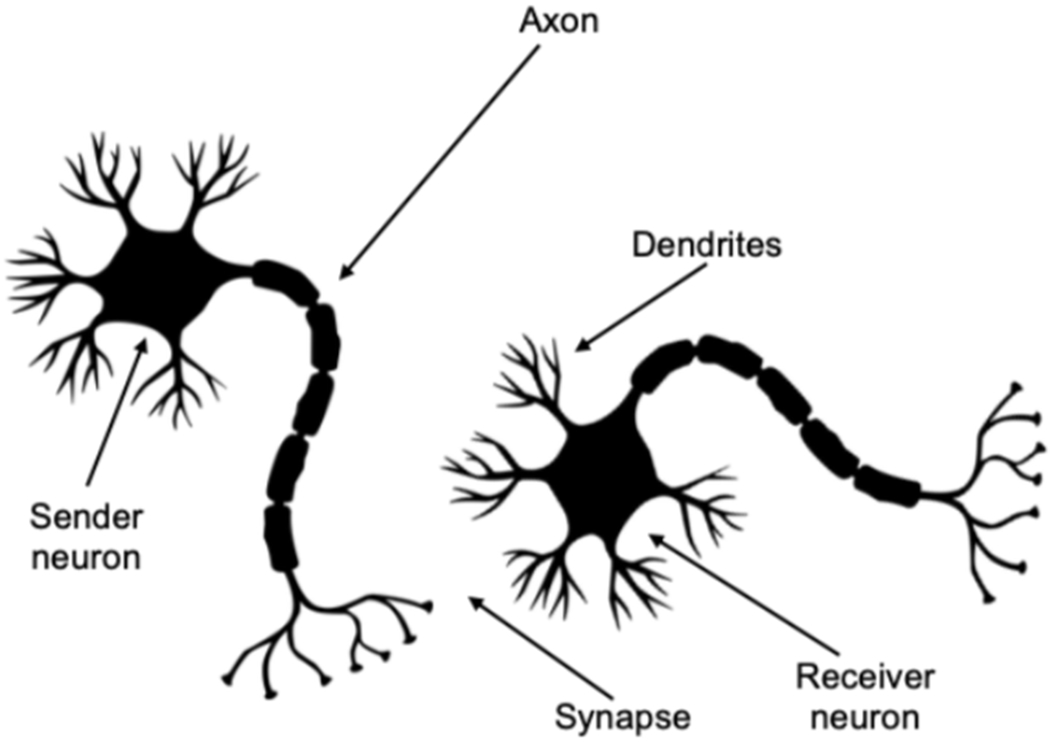
\includegraphics[width=0.65\textwidth]{figs/neuron-communication.jpg}
    \caption{Communication between neurons}
    \label{fig:neuron-communication}
\end{figure}

Alzheimer's Disease intervenes in this process by gradually decreasing the utility function of each neuron, leading to
the atrophy of the brain's proficiencies, as neurons imminently die one by one.

There are three major factors included in the dynamic between AD and neurons.
First of all, a key advantage of neurons which many other cells lack, and which accomplishes
their long survival, is the ability to repair themselves, form new connections, or changing current ones' magnitude.
Secondly, synaptic connections, which solidify the signal transmission process, and lastly the intake of glucose and
oxygen necessary for their normal functioning.
It is believed these fundamental attributes of a healthy human receive considerable drawbacks upon the disease's presence.
\cite{NIH1}

\subsection{Causes} %* -- Introduction/Causes
While the factors which lead to Alzheimer's Disease are not yet properly understood, past research and studies prove that some
of the most commonly met criterias which lead to a diagnostic include genetic inheritance - chances of developing Alzheimer's
Disease increase by 30\% when another close relative suffers from it \cite{HMS20192801}, lifestyle and environmental factors.

\subsubsection*{Genetical Inheritance} %* -- Introduction/Causes/GeneticalInheritance
Genes represent instructions passed down from generation to generation, which contain information regarding how various cells
need to behave. Some roles played by these include defining one's height, or the color of hair and eyes.

Advances in genetic research have led to discover 80 genetic areas that can possibly play a part in AD development \cite{NIH2}.
One of the more known genes which raises the risk of Alzheimer's Disease is the apolipoprotein E (APOE) gene, which comes in forms such as
$\epsilon_2, \epsilon_3, \epsilon_4$. A pair of two such APOE genes, one from each parent, gets passed down to the next generation
resulting in 6 possible cases. Among them, the $\left(\epsilon_4,\epsilon_4\right)$ combination having the highest risk of AD,
only increasing, not guaranteeing it, and in contrast, $\epsilon_2$ provides a higher degree of protection against it.

\subsubsection*{External Factors} %* -- Introduction/Causes/ExternalFactors
Besides genetical inheritance, researchers have drawn conclusions regarding causes of Alzheimer's Disease to contain a plethora
of other outside factors, which we can have a higher influence on.
Among these can be found vascular conditions - high blood pressure, heart diseases - and metabolic diseases - obesity and diabetes
\cite{NIH2}.

%* todo - 15/04 -> symptoms, process of diagnosios, how scans work
\subsection{Symptoms} %* -- Introduction/Symptoms
Before beginning the discussion about its effects, a noteworthy fact is that brain structure modifications, whether they may be
neurofibrillary tangles or plaques of amyloid, occur several years before any cognitive issues manifest at all, a stage of the disease titled
preclinical. With that being said, their presence does not inevitably lead to dementia.

Apart from preclinical stage, AD has been classified into three others: mild, moderate, severe.

\subsubsection*{Early-stage (Mild)} %* -- Introduction/Symptoms/Early-stage
A person which suffers from early-stage Alzheimer's Disease can still function normally on their own, without mandatory outside benefactors.
However, changes appear in memory skills, starting to forget recently gained information, such as names at social gatherings, objects placements
and losing the reasoninng behind starting certain activities.

It is important to understand these memory setbacks are hardly noticeable by the affected one, more commonly than not leaving it up to their
surrounding group of people and friends to pinpoint them and initiate medical visits.

\subsubsection*{Middle-stage (Moderate)} %* -- Introduction/Symptoms/Middle-stage
Here, over the course of many years, cognitive skills start degrading, with the diagnosed person needing increasing help from other people.
Previous rare memory losses become the norm, and even more proeminent. Not only that, disturbances in emotions begin escalating, some
expressed in a stronger tone, while others hardly able to be exhibited at all.

Daily tasks must be simplified to the level the person with Alzheimer's can accomplish them, and as the external attention needed rises,
place them in special care centers where experienced caretakers can easily reach out.

\subsubsection*{Late-stage (Severe)} %* -- Introduction/Symptoms/Late-stage
This final stage of AD is categorized by vital losses in the ability to function at all. Patients stop reacting to outside factors
altogether, and even initiating conversations. In due course, pain becomes impossible to verbalize, and as such, hourly check-ups
are necessary. \cite{AA1}

\subsection{Diagnosis Process} %* -- Introduction/DiagnosisProcess
AD diagnosis can only be carried out upon gathering a variety of complex data, which includes medical history, assessments of
cognitive and physical skills, neurological exams, brain scans, blood tests and cerebrospinal fluid.

Medical history consists of modifications in how the patient behaves over the course of time, past and present medical concerns
and even the undergoing medication. Other than these, information about other family members' health conditions is obtained, since,
as previously mentioned, genes do play a role in increasing the risk, or protecting against Alzheimer's Disease.

An overall health status is evaluated, involving commonly met questions about diet, blood pressure and pulse, checking
the quality of breathing and sample taking for testing.

Cognitive tests' purpose is to express a general view whether memory impairment takes a toll in the daily life of the diagnosed,
and to shed light on the awareness of the disease. A number of tests are simple - tasks of remembering sequences of words, or
mathematic operations, but there also exist those that take a longer period of time, alongside with raised levels of attention.

The neurological examination typically implies assessing the patient's nervous system, where a physician tries to distinguish
between the possibilities of the disease to be a different brain disorder instead of AD - brain tumors or Parkinson's Disease.

Brain imaging is used to form 3D and 2D, functional and structural scans of the brain, through which experts can point out
characteristics specific to Alzheimer's Disease. One such mark is the presence of higher concentrations than normal of amyloid
beta ($A\beta $ or Abeta), peptides considered the essential part of amyloid plaques. This specific part of the diagnosis
process typically serves only as a last resort. \\
\cite{AA2}

%* todo: fix this shit sometimes, sounds awful

\subsection{Imaging Modalities Involved in Alzheimer's Disease} %* -- Introduction/ImagingModalitiesInvolved
Through recent technological advancements, brain imaging's role has shifted to a crucial one. By and large, imaging has
expanded into various different modalities, each with their own strengths and weaknesses, but combined lead to a better
analysis of AD's effects on the human brain. \cite{Johnson2012BrainII}

\subsubsection*{Amyloid PET} %* -- Introduction/ImagingModalitiesInvolved/AmyloidPET
Amyloid Positron Emission Tomography is a non-invasive technique, which locates amyloid plaques.
Due to its unavailability and expensive price, this method has not seen much popularity, but
there is no denying its accuracy, past studies showing that 96\% of the people who had performed an
amyloid PET scan and were amyloid positive had been diagnosed with Alzheimer's Disease.\\
\cite{Johnson2012BrainII}

\begin{figure}[htbp]
    \centering
    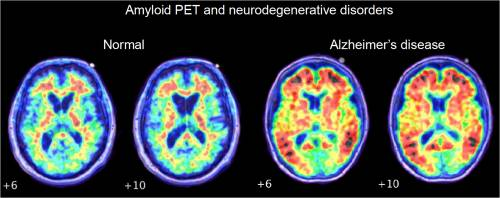
\includegraphics[width=0.65\textwidth]{figs/amyloid-pet.jpeg}
    \caption{Amyloid PET images}
    \label{fig:amyloid-pet}
\end{figure}

\subsubsection*{FDG PET} %* -- Introduction/ImagingModalitiesInvolved/FDG-PET
Fluoro-deoxy-D-glucose (FDG) PET showcases synaptic activity, because the brain's primary energy comes from glucose.
The Fluorine part of the FDG comes as a consequence of the convenient dynamic it has with Positron Emission Tomography,
which easily detects it.

\begin{figure}[htbp]
    \centering
    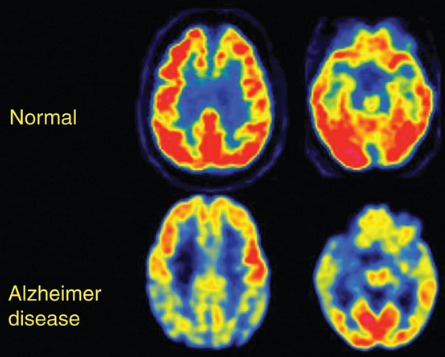
\includegraphics[height=0.2\textheight,width=0.40\textwidth]{figs/fdg-pet.png}
    \caption{Transitional FDG-PET scans}
    \label{fig:fdg-pet}
\end{figure}

\subsubsection*{Structural MRI} %* -- Introduction/ImagingModalitiesInvolved/SMRI
Structual Magnetic Resonance Imaging (sMRI) is a non-invasive method applied to observe pathology and anatomy of the brain
by emitting radiofrequency pulses in sequences. Its main purpose is to exhibit brain atrophy, associated with shrinking size
due to neuron counts declining. One of its drawbacks is that, compared to PET imaging, hallmarks of AD cannot be detected,
and also atrophy isn't specific to the disease discussed.

\subsubsection*{Functional MRI} %* -- Introduction/ImagingModalitiesInvolved/FMRI
As the previous method, the functional variant of MRI is non-invasive as well, but, on the other hand, provides
scientists a neuronal activity mapping of the brain. A few of them require the patient to perform certain cognitive tasks
during the scanning process, and there are also some which need the brain to be found in a specific resting state.
Functional MRI's setback is the necessity of lack of motion, and any of the patient's movements could lead to faulty
data.

%* todo 16/4 -> fix intro(imaging), kinda day off
% todo 17/4 -> describe prediction tasks, history of approaches, how neural networks work, start related works, at least 1 papers described 

\subsection*{Tasks}
An important question to ask before traversing further, is what type of predictions are we demanding from ourselves?
As aforementioned, Alzheimer's Disease classifies itself in three stages: Normal Cognition(NC), Mild Cognitive Impairment(MCI)
- which further breaks down into progressive MCI and stable MCI, pMCI and sMCI respectively - and Alzheimer's Disease.

These various disease progressions have given birth to a collection of tasks for researchers. There are approaches
which classify AD in two - NC vs AD, NC vs MCI, MCI vs AD -, three - NC vs MCI vs AD - and even four classes, including MCI's
subclasses. On the other hand, regression problems build the percentage of a specific stage to progress.

\subsection*{Deep Learning}
Recent advancements in deep learning, with a higher degree of respect to Convolutional Neural Networks (CNNs) and Recurrent
Neural Networks(RNNs), have had main roles in raising the speed and accuracy with which classification or regression task
are accomplished.

Before 2013, the most commonly met algorithms included stacked Restricted Boltzmann machines and stacked autoencoders,
but ever since, CNNs and RNNs have taken the spotlight, surprising the world with their results, especially when given
inputs of MRI or PET \cite{make6010024}.

Deep Learning's key characteristic is the power to find a hypothesis leading to the desired outcome unbeknownst to the
humans of how it is realized, with the drawback of needing a high amount of data and proportionate computational resources.

\subsubsection*{Artificial Neural Networks}
As their name suggests, ANNs consist of a collective of artifical neurons connected between eachother. They represent how
researchers have tried to emmulate the biological neural brain, where the nodes play the role of neurons, and connections,
or edges, between them that of synapses.

Furthermore these neurons are stratified into various layers, through which information passes, notably the initial and last
layer have been titled as input and output accordingly, while the ones in-between called hidden layers.

Each neuron's meaning is to receive information and process it in order to be passed to the next layer through the
array of synapses. Activation functions take place in the processing stage, in order for non-linearities to be applied
to the hypothesis being built.

In the course of multiple iterations, these neurons adapt to the task given by the designer, adaptation formally known as weights.

\subsubsection*{Convolutional Neural Networks}
These types of artifical neural networks are feedforward - input flows only in forward direction, without loops - and exhibit
the capacity to extract features automatically. In such networks, convolutional layers and pooling layers represent
their main components. Convolutional layers transform the data by passing it through a kernel creating a feature map
, and pooling layers finetune network parameters by taking these feature maps and reducing their size.
This final product also takes the name of pooled feature map \cite{li2021survey}.

\subsubsection*{Recurrent Neural Networks}
RNNs are the other types of neural networks, described best by how information propagates inside it, which compared to
the single directioned CNNs, RNNs are bi-directional. This property creates the opportunity of some information to be
used in more than just one place, with the justification that evaluations sometimes show improvements in results.


\subsection{Regions of Interests}
This section serves as a guide to understanding why certain regions of the brain deserve more attention than others while
studying the Alzheimer's Disease.

\subsubsection*{Medial Temporal Lobe (MTL)}
MTL represents a brain region known for its capacities of handling memory abilities related to space and episodes \cite{10.3389/fnsys.2017.00019}.
Previous works prove that it is among the first to suffer from shrinkage over the course of AD's effect \cite{deFlores2131}, \\
mainly due to how soon tangles of neurofibrilaries develop (NFT). Upon the beginning of NFTs, they start spreading further in the network,
ultimately reaching the neocortex, region which realizes reasoning, meaning and consciousness.

\begin{figure}[htbp]
    \centering
    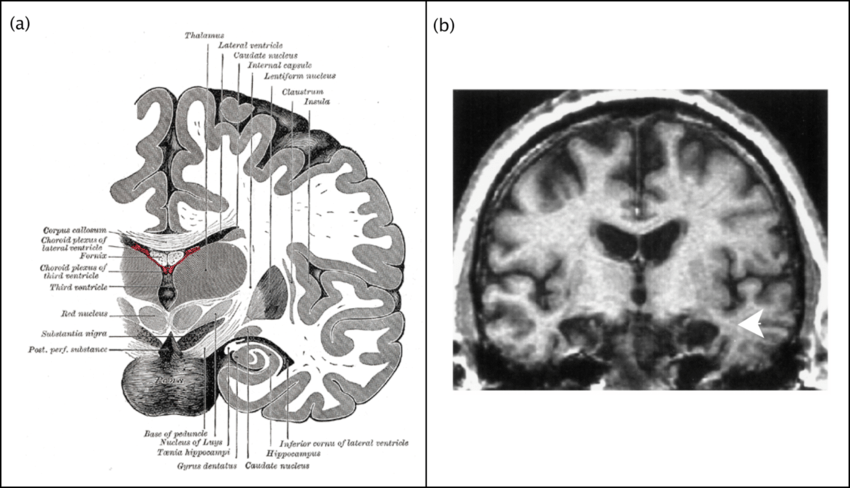
\includegraphics[height=0.25\textheight,width=0.7\textwidth]{figs/MTL-coronal.png}
    \caption{(a) Illustration showing the location of medial temporal lobe structures on coronal section
        (taken from Gray's Anatomy). (b) Coronal T1-weighted MRI scan of HM's brain, showing the absence of the
        hippocampus and related medial temporal lobe structures bilaterally (arrowhead). Source: \cite{MTL-image}}
    \label{fig:MTL}
\end{figure}


% todo 18/04 -> 2 3D-MRI CNN, 2 RNN approaches
\newpage
\newpage

\section{Related Work} %* -- RelatedWork
\cite{bae2020} suggest a Convolutional Neural Network approach where, in contrast to other CNN approaches, they give as input
2D-MRI scans, with attention to the medial temporal lobe (MTL) from coronal slices, MTL being widely considered to be the
area suffering most change. Even though other parts of the brain contain valuable information as well, they deem it
unnecessary due to probabilities of altering the algorithm's outcomes. They make use of ADNI\footnote{Alzheimer's Disease Neuroimaging Initiative}
and SNUBH\footnote{Seoul National University Bundang Hospital} datasets in order to highlight the importance of each patient's background for
the predictions, such as ethnicity and educational levels, by which the human brain is thought to vary accordingly.
Their approach include evaluations through AUC (area under the receiver operating characteristic curve), accuracy, sensitivity and specificity
- for ADNI: 88\%, 83\%, 76\%, 89\%, and for SNUBH: 89\%, 82\%, 79\%, 85\% . They have also underwent within and between dataset comparisons,
having used 2 datasets: 91\%-94\% for within-dataset and 88\%-89\% for between.

On the other hand, \cite{PMID-31201098} provide a 3D-MRI approach using CNNs where the a region of the medial temporal lobe
is taken into consideration this time, the hippocampus. The used datasets include 3 stages from the ADNI study: 1, GO \& 2 and
the AIBL\footnote{Australian Imaging Biomarkers and Lifestyle Study of Aging}. Their main concern is that of predicting the
progression from the moderate to servere stage along with a time estimation, underlining that previous MCI and AD comparisons
only classify MCI in either progressive (pMCI) or stable (sMCI). Accuracies for each dataset are the following: ADNI with
76.2\%, AIBL with 78.1\%.

\cite{10.1117/1.JMI.8.2.024503} realize multiple trials with different architectures and input modalities, 2D and 3D MR scans,
however making use only on a small amount of 132 subjects from the ADNI dataset before dividing in the corresponding purposes
to the algorithm. Their best results come from SqueezeNet and ResNet-18 on 2D inputs using transfer learning.
For measurements of accuracy, sensitivity and specificity, ResNet had achieved 84.38\%, 87.5\%, 81.25\% respectively, while
SqueezeNet's results were 90.62\%, 81.25\% and 100\%.

% todo 19/04 -> explain medial temporal lobe, 1-2 more articles

Nguyen and colleagues tackled a Recurrent Neural Network method for the TADPOLE\footnote{The Alzheimer's Disease Prediction
    Of Longitudinal Evolution} Challenge \cite{NGUYEN2020117203}. \\
Corresponding to the competition's recommendation, a set of 23 variables was used as inputs which included multi-modal
imaging, cognitive test results and clinical diagnosis. The research had tested the minimalRNN architecture \cite{Chen2017MinimalRNNTM}
which was modified properly in order for the problem to become 6-class labeling problem: NC stable, NC progressive, MCI recovered,
MCI stable, MCI progressive and AD stable. Their trials were verified using multiclass area under the curve (mAUC) and balanced
class accuracy (BCA) with the scores of 94.5\% and 88\%. One of their unique noteworthy contribution is their ways of
handling missing data at consecutive time points, which consisted of three variations: firstly, model-filling, done by the model
during training and testing, and the next two were considered as preprocessing techniques: forward-filling and linear-filling using linear
interpolation. Model-filling coming out on top for the minimalRNN solution.

\newpage
\section{Setup Summary(will be replaced later)}
\begin{itemize}
    \item 2D-MR image CNN approach
    \item Classify between NC and AD
    \item AUC, accuracy, specificity and sensitivity as evaluation metrics.
    \item Dataset: ADNI (available upon request from \url{https://adni.loni.usc.edu/}).
    \item Tools: python, pytorch.
    \item Why? - 2D mr scans can lead to more complex CNN networks, while still having less parameters than 3D CNN
\end{itemize}


% todo 21/04 code/dataset handling
\newpage
\section{Dataset handling}
The data used in this research has been taken from the Alzheimer's Disease Neuroimaging Initiative (ADNI)
database (adni.loni.usc.edu). The initiative started in 2003 led by Principal Investigator Michael W. Weiner, MD
as a public-private partnership. Its primary objective has been to verify if serial magnetic resonance imaging (MRI),
positron emission tomography (PET), clinical and neuropsychological assessments, as well as other biological markers
can together measure the progression of mild cognitive impairment (MCI) and early Alzheimer's Disease (AD)\\
\cite{PMID20042704}

% todo: fix here later, made really early for a stupid assignment
Images are taken using structural MR imaging (sMRI) which display brain atrophies. These scans can be found in
NiFTi format (.nii) and using the \textit{nibabel} library in python, which was designed for the purpose of
supporting neuroimaging file formats, they can be accessed and plotted as 2D images, according to a specific
plane - coronal, sagittal or axial (Fig \ref{fig:images}).

\begin{figure}[htbp]
    \centering
    \begin{subfigure}[b]{0.3\textwidth}
        \centering
        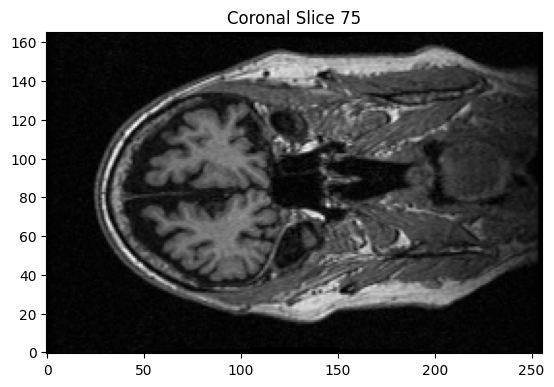
\includegraphics[width=\textwidth, height=0.16\textheight]{figs/coronal-slice-75.png}
        \caption{Coronal Slice}
        \label{fig:sub1}
    \end{subfigure}
    \begin{subfigure}[b]{0.3\textwidth}
        \centering
        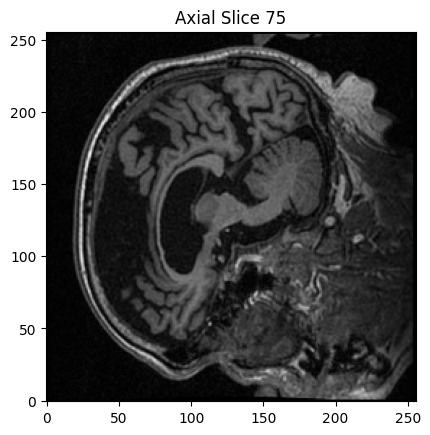
\includegraphics[width=1\textwidth, height=0.16\textheight]{figs/sagittal-slice-75.png}
        \caption{Sagittal Slice}
        \label{fig:sub2}
    \end{subfigure}
    \begin{subfigure}[b]{0.3\textwidth}
        \centering
        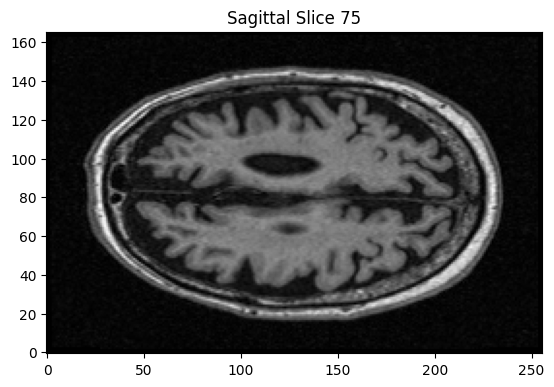
\includegraphics[width=\textwidth, height=0.16\textheight]{figs/axial-slice-75.png}
        \caption{Axial Slice}
        \label{fig:sub3}
    \end{subfigure}
    \caption{Visualisation of an sMRI scan}
    \label{fig:images}
\end{figure}

Firstly, as a preprocessing step, skull-stripping is applied, which is realized by applying a segmentation mask
to the normal untouched versions of the MRI. This has been provided by the ADNI, and so only the algorithm
needs to be applied.

\begin{figure}[htbp]
    \centering
    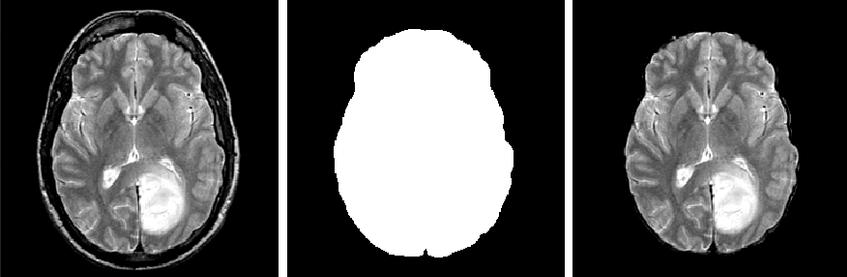
\includegraphics[height=0.16\textheight,width=0.7\textwidth]{figs/segmentation-mask.png}
    \caption{Skull-stripping using a segmentation mask}
    \label{fig:segm-mask}
\end{figure}

\newpage
\section{Acknowledgements}

This work is the result of my own activity, and I confirm I have neither given, nor received unauthorized assistance for this work.

I declare that I did not use generative AI or automated tools in the creation of content or drafting of this document.


Data collection and sharing for the Alzheimer's Disease Neuroimaging Initiative (ADNI) is funded by the National
Institute on Aging (National Institutes of Health Grant U19 AG024904). The grantee organization is the Northern
California Institute for Research and Education. In the past, ADNI has also received funding from the National
Institute of Biomedical Imaging and Bioengineering, the Canadian Institutes of Health Research, and private
sector contributions through the Foundation for the National Institutes of Health (FNIH) including generous
contributions from the following: AbbVie, Alzheimer’s Association; Alzheimer’s Drug Discovery Foundation;
Araclon Biotech; BioClinica, Inc.; Biogen; Bristol-Myers Squibb Company; CereSpir, Inc.; Cogstate; Eisai Inc.;
Elan Pharmaceuticals, Inc.; Eli Lilly and Company; EuroImmun; F. Hoffmann-La Roche Ltd and its affiliated
company Genentech, Inc.; Fujirebio; GE Healthcare; IXICO Ltd.; Janssen Alzheimer Immunotherapy Research \&
Development, LLC.; Johnson \& Johnson Pharmaceutical Research \&Development LLC.; Lumosity; Lundbeck;
Merck \& Co., Inc.; Meso Scale Diagnostics, LLC.; NeuroRx Research; Neurotrack Technologies; Novartis
Pharmaceuticals Corporation; Pfizer Inc.; Piramal Imaging; Servier; Takeda Pharmaceutical Company; and
Transition Therapeutics.
\newpage

\bibliographystyle{plainnat}
\bibliography{references}


\end{document}
